% Copyright 2009 by Tomasz Mazur
%
% This file may be distributed and/or modified in all ways.

%\documentclass[xcolor=pdftex,t,11pt]{beamer}
\documentclass[xcolor=pdftex,t,11pt,handout]{beamer}

%%%%%%%%%%%%%%%%%%%%%%%%%%%%%%%%%%
%       SET OPTIONS BELOW        %
%%%%%%%%%%%%%%%%%%%%%%%%%%%%%%%%%%
\usepackage[icelandic, english]{babel}
\usepackage{t1enc} 
\usepackage{textcomp}
\usepackage[
% Toggle showing page counter
pagecounter=true,
%
% String to be used between the current page and the
% total page count, e.g. of, /, from, etc.
pageofpages=of,
%
% Defines the shape of bullet points. Available options: circle, square
bullet=circle,
%
% Show a line below the frame title. 
titleline=true,
%
% Set the style of the title page (true for fancy, false for standard)
alternativetitlepage=true,
%
% Institution logo for fancy title page.
% Comment out to remove the logo from the title page.
% IMPORTANT: THERE IS A BUG IN SOME VERSIONS OF PDFLATEX AND FONTS
% ON THE LOGOS ARE NOT RENDERED PROPERLY. IN SUCH A CASE ADD `2` 
% TO THE NAME OF THE LOGO, E.G. comlab2 INSTEAD OF comlab
titlepagelogo=../hilogo,
%
% Department footer logo for fancy title page
% Comment out to remove the logo from the footer of the title page/
% IMPORTANT: THERE IS A BUG IN SOME VERSIONS OF PDFLATEX AND FONTS
% ON THE LOGOS ARE NOT RENDERED PROPERLY. IN SUCH A CASE ADD `2` 
% TO THE NAME OF THE LOGO, E.G. comlab2 INSTEAD OF comlab
%titlepagefooterlogo=images/titlepage/comlab,
%
% Institution/department logo for ordinary slides
% Comment this line out to remove the logo from all the pages.
% Available logos are: ou, comlab, comlabinline, comlabou
% IMPORTANT: THERE IS A BUG IN SOME VERSIONS OF PDFLATEX AND FONTS
% ON THE LOGOS ARE NOT RENDERED PROPERLY. IN SUCH A CASE ADD `2` 
% TO THE NAME OF THE LOGO, E.G. comlab2 INSTEAD OF comlab
ordinarypageslogo=../hilogoname,
%
%
% Add watermark in the bottom right corner
%watermark=<filename>,
%
% Set the height of the watermark.
%watermarkheight=100pt,
%
% The watermark image is 4 times bigger than watermarkheight.
%watermarkheightmult=4,
]{../beamerthemeTorino} 

% Select color theme. Available options are:
% mininmal, greenandblue, blue, red
\usepackage{../beamercolorthemehi}

%Select different font themes.Available options are:
% default, serif, structurebold, structureitalicserif, structuresmallcapsserif
\usefonttheme{structurebold}

\setbeamercovered{transparent}
\usepackage{tabularx}

\usepackage{natbib} %citep and citet
%\bibpunct[:]{(}{)}{;}{a}{}{,}
%\renewcommand{\bibsection}{\subsubsection*{\bibname } }

\newcommand{\bi}{\begin{itemize}\item}
\newcommand{\ei}{\end{itemize}}

\usepackage{latexsym}
\usepackage{amsmath,bm,amssymb}

\usepackage[colorinlistoftodos]{todonotes}
\usepackage{comment}
\usepackage{multirow}
\usepackage{rotating}
\usepackage{longtable}
\usepackage{paralist}
\usepackage[perpage,symbol*]{footmisc}
\usepackage{tabu}
\usepackage{tabularx}
\newcommand{\tcr}[1]{{\color{red} #1}}
\newcommand{\tcb}[1]{{\color{blue} #1}}
\newcommand{\tcg}[1]{{\color{green} #1}}

\usepackage{paralist}


%\renewcommand{\rho}{{\varrho}}

\renewcommand{\vec}[1]{\mathbf{#1}}
\newcommand{\vphi}{{\boldsymbol{\phi}}}
\newcommand{\Exp}{{\mathbb E}}
\newcommand{\inner}[2]{\big<{#1}\cdot{#2}\big>}
\newcommand{\norm}[1]{\lVert#1\rVert}

\newcommand{\vsigma}{{\vec{\sigma}}}
\newcommand{\mat}[1]{\mathbf{#1}}
\newcommand{\R}{{\mathbb R}}
\newcommand{\strng}[1]{{\mbox{\tt #1}}}
\newcommand{\abs}[1]{\lvert#1\rvert}
\newcommand{\argmax}{\mathop{\rm argmax}}
\newcommand{\argmin}{\mathop{\rm argmin}}


\hyphenpenalty=750
\hyphenation{heur-ist-ics}
\hyphenation{algo-rithm}

% job-related
\newcommand{\phiproc}{$\phi_1$}
\newcommand{\phistartTime}{$\phi_2$}
\newcommand{\phiendTime}{$\phi_3$}
\newcommand{\phiwrmJob}{$\phi_4$}
\newcommand{\phiwait}{$\phi_5$}
\newcommand{\phiarrivalTime}{$\phi_6$}
\newcommand{\phijobOps}{$\phi_7$}
% mac-related
\newcommand{\phimac}{$\phi_8$}
\newcommand{\phimacFree}{$\phi_9$}
\newcommand{\phiwrmMac}{$\phi_{10}$}
\newcommand{\phimacOps}{$\phi_{11}$}
% flow-related
\newcommand{\phislotCreated}{$\phi_{12}$}
\newcommand{\phislotReduced}{$\phi_{13}$}
\newcommand{\phislots}{$\phi_{14}$}
\newcommand{\phislotsTotal}{$\phi_{15}$}
% schedule related
\newcommand{\phimakespan}{$\phi_{16}$}
\newcommand{\phiwrmTotal}{$\phi_{17}$}
\newcommand{\phitotProc}{$\phi_{18}$}
\newcommand{\phistep}{$\phi_{19}$}
% global
\newcommand{\phiMWR}{$\phi_{20}$}
\newcommand{\phiLWR}{$\phi_{21}$}
\newcommand{\phiSPT}{$\phi_{22}$}
\newcommand{\phiLPT}{$\phi_{23}$}
\newcommand{\phiRND}{$\phi_{24}$}


\usepackage{cleveref} % must come last! 
 % put your own shorthand declarations in this document
%%%%%%%%%%%%%%%%%%%%%%%%%%%%%%%%%%
%       PRESENTATION INFO        %
%%%%%%%%%%%%%%%%%%%%%%%%%%%%%%%%%%

\author{Helga Ingimundard\'{o}ttir\\Thomas Philip Runarsson}
\title{Supervised Learning Linear Composite Dispatch Rules for Scheduling}
\subtitle{Case study for JSP and PFSP}
\institute{University of Iceland}	
\date{April 22$^{nd}$, 2013}


\begin{document}


%%%%%%%%%%%%%%%%%%%%%%%%%%%%%%%%%%
%       SLIDE DEFINITIONS        %
%%%%%%%%%%%%%%%%%%%%%%%%%%%%%%%%%%

\begin{frame}[plain]
	\titlepage
\end{frame}

\frame{
\frametitle{Outline}
\tableofcontents[part=0] % part=0, sectionstyle=show/shaded
}

\section{Introduction}
\frame{\tableofcontents[currentsection]}

\frame{
\frametitle{Motivation}

\begin{block}{General Goal}
\begin{itemize} 
\item General goal is how to search for \emph{good} solutions for an arbitrary problem domain. 
\item Automate the design of optimization algorithms. 
\item Use of randomly sampled problem instances and their corresponding optimal vs. suboptimal solutions.
\end{itemize}
\end{block}
}

\frame{\frametitle{Case Study: JSP and PFSP}
\begin{block}{Abstract}
\begin{itemize}
\item Framework for creating dispatching rules for JSP and PFSP.
\item Supervised learning based on optimal and sub-optimal solutions. 
\item Training data is randomly generated problem instances and their optimal solutions. Method is purely \alert{data-driven}.
\item \alert{Linear classification} to identify good dispatches from worse ones.
\item \alert{Robust} for higher dimensions. 
\end{itemize}
\end{block}
\textbf{Keywords:} Scheduling $\bullet$ Composite dispatching rules $\bullet$ JSP  $\bullet$ PFSP $\bullet$ Generating training data $\bullet$ Sampling $\bullet$ Ranking $\bullet$ Scalability $\bullet$ Ordinial Regression $\bullet$ Evolutionary Search
}


\section{Job Shop Scheduling}
\frame{\tableofcontents[currentsection]}

\frame[allowframebreaks]{
\frametitle{Job Shop Scheduling}
\begin{block}{JSP}
	Simple job shop scheduling problem  is where $n$ jobs are scheduled on a set of $m$ machines, subject to constraints:
	\begin{itemize}
	\item each job must follow a predefined machine order,
	\item that a machine can handle at most one job at a time.
	\end{itemize}
	
	\textbf{Objective:} schedule the jobs so as to minimize the maximum completion time, i.e. makespan, $C_{\max}$.
\end{block}
\begin{block}{PFSP}	
    Permutation flow shop scheduling is the same as JSP except the predefined machine order is homogeneous for all jobs.	
\end{block}
%\begin{itemize}
%	\item Job $j$ has an indivisible operation time on machine $a$, $p(j,a)$, which is assumed to be integral, where $j \in\{1,..,n\}$ and $a\in\{ 1,..,m\}$. 
%	\item Job $j$ has a specified processing order through the machines, it is a permutation vector, $\sigma_j$, of $\{1,..,m\}$, i.e. $j$ can be processed on $\sigma_j(a)$ only after it has completed on $\sigma_j(a-1)$.
%	\begin{itemize} \item Permutation flow shop scheduling (PFSP) is when $\sigma_j$ is fixed $\forall j$. \end{itemize}
%\end{itemize}
\begin{block}{Problem space distributions used in experimental studies}
\begin{table}\centering
{\scriptsize \renewcommand{\arraystretch}{0.6}
\begin{tabular}{|l|l|c|c|c|l|}\hline 
type&name&size ($n\times m$)& $N_{\text{train}}$&$N_{\text{test}}$  & note 
\\ \hline\hline 
\multirow{4}{*}{JSP}
&$\mathcal{P}_{jrnd}^{6\times5}$ & $6\times5$ & 500 & 500 & random \\
&$\mathcal{P}_{jrndn}^{6\times5}$ & $6\times5$ & 500 & 500 & random-narrow \\
&$\mathcal{P}_{jrnd}^{10\times10}$ &$10\times10$& -- & 500 & random \\
&$\mathcal{P}_{jrndn}^{10\times10}$ &$10\times10$& -- & 500 & random-narrow \\ \hline\hline 
\multirow{6}{*}{PFSP}
&$\mathcal{P}_{frnd}^{6\times5}$ &$6\times5$& 500&500& random \\ 
&$\mathcal{P}_{frndn}^{6\times5}$&$6\times5$& 500&500& random-narrow \\ 
&$\mathcal{P}_{fjc}^{6\times5}$  &$6\times5$& 500&500& job-correlated \\ 
&$\mathcal{P}_{frnd}^{10\times10}$ &$10\times10$&--&500&random \\ 
&$\mathcal{P}_{frndn}^{10\times10}$&$10\times10$&--&500& random-narrow \\ 
&$\mathcal{P}_{fjc}^{10\times10}$  &$10\times10$&--&500& job-correlated \\ 
\hline
\end{tabular}
}
\end{table}

\end{block}

\framebreak
\begin{block}{Simple Priority Dispathcing Rules}
\begin{figure} \centering
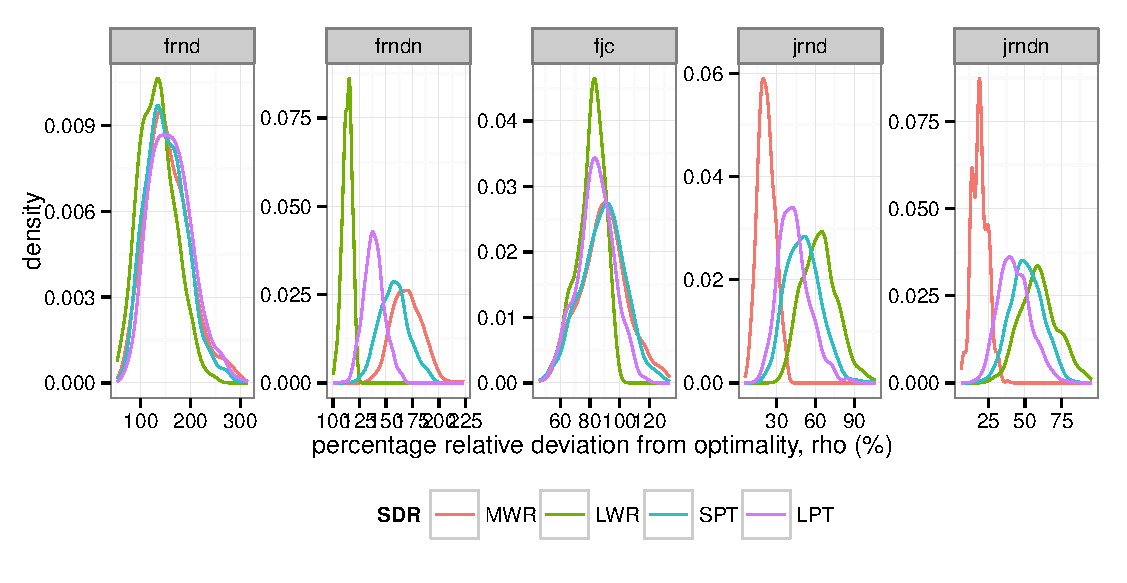
\includegraphics[width=0.8\textwidth]{figures/SDR10x10color}
\end{figure}
\end{block}



\begin{block}{Dispatching rules (DR) for constructing JSSP}
\begin{itemize}
	\item Starts with an empty schedule and adds on one job at a time. 
	\item When a machine is free the DR inspects the waiting/available jobs and selects the job with the \alert{highest priority}. 
	\item Complete schedule consists of $\ell=n\times m$ sequential dispatches.
	\item At each dispatch $k$ features $\vphi(k)$ for the temporal schedule are calculated.
	\item Performance of DR is compared with its optimal makespan, as percentage relative deviation from optimality: $\rho=\frac{C_{\max}^{DR}-C_{\max}^{opt}}{C_{\max}^{opt}}\cdot 100\%$
\end{itemize}
\end{block}

\begin{block}{Features for JSSP}
\begin{table}[t!]
 {\scriptsize
 \begin{center}
  \begin{tabular}{|c|l|}
   \hline\hline
  $\vphi$ & Feature description \\ \hline
  $\phi_1$ & processing time for job on machine\\
  $\phi_2$ & start-time \\
  $\phi_3$ & end-time \\
  $\phi_4$ & when machine is next free \\
  $\phi_5$ & current makespan \\
  $\phi_6$ & work remaining \\
  $\phi_7$ & most work remaining \\
  $\phi_8$ & slack time for this particular machine \\
  $\phi_9$ & slack time for all machines \\
  $\phi_{10}$ & slack time weighted w.r.t. number of operations already assigned \\
  $\phi_{11}$ & time job had to wait\\
  $\phi_{12}$ & size of slot created by assignment \\
  $\phi_{13}$ & total processing time for job \\
 \hline\hline
  \end{tabular}
 \end{center}}
\end{table}
\end{block}
}

\frame{
\frametitle{Job Shop Scheduling}
\begin{example}
	\begin{center}
		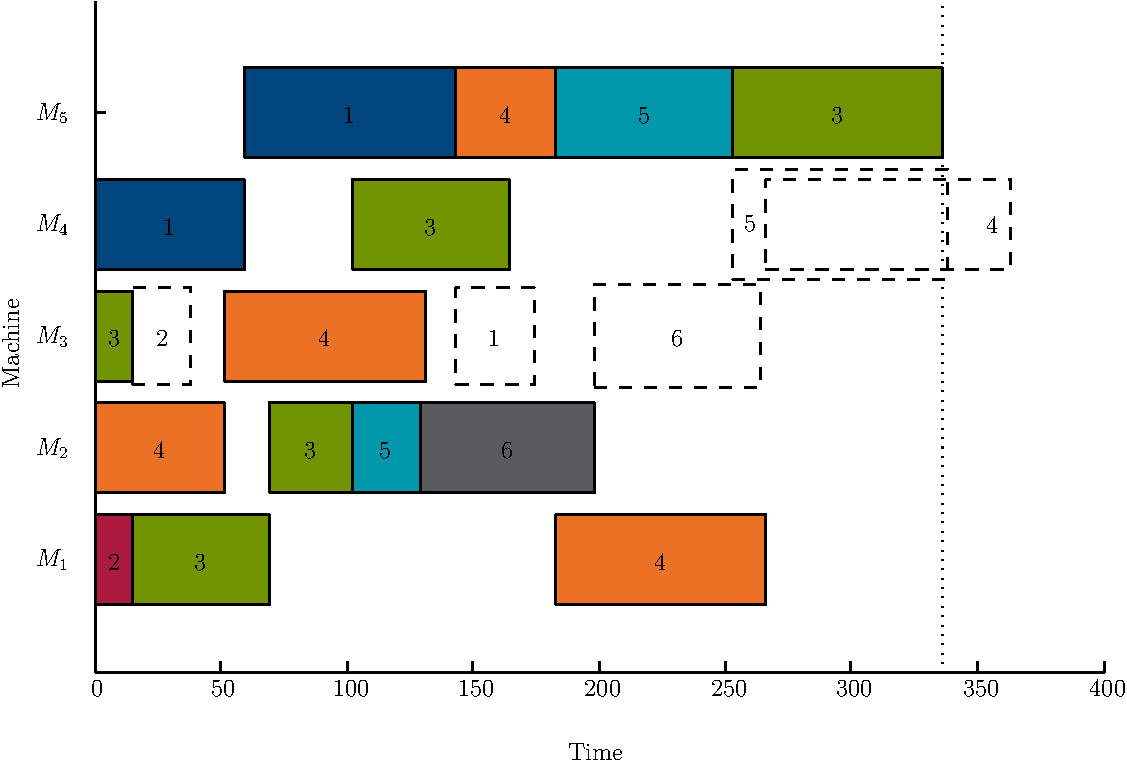
\includegraphics[width=0.5\columnwidth]{figures/jssp_example}
	\end{center}
	A schedule being built at step $k=16$. The dashed boxes represent five different possible jobs that could be scheduled next using a DR.
\end{example}
}

\section{Preference models}
\frame{\tableofcontents[currentsection]}

\frame[allowframebreaks]{\frametitle{Ordinal Regression}
\begin{block}{Preference learning problem}
Specified by a set of \alert{preference pairs}:
\begin{equation*}
S = \left\{\left\{\vec{z}_o,+1)\right\}_{k=1}^{\ell},\left\{\vec{z}_s,-1)\right\}_{k=1}^{\ell}
\;|\;\forall o\in \mathcal{O}^{(k)},s\in \mathcal{S}^{(k)}
\right\}\subset \Phi\times Y \label{eq:S}
\end{equation*}
where the set of point/rank pairs are:
\bi Optimal decision: $\vec{z_o}=\vphi^{(o)}-\vphi^{(s)}$, ranked $+1$
\item Sub-optimal decision: $\vec{z_s}=\vphi^{(s)}-\vphi^{(o)}$, ranked $-1$
\ei
\end{block}
\framebreak

\bi Mapping of points to ranks: $ \{h(\cdot) : \Phi \mapsto Y\}$ where 
\begin{equation}
\vphi_o \succ \vphi_s \quad \Leftrightarrow \quad h(\vphi_o) > h(\vphi_s) \nonumber
\end{equation}

\item The preference is defined by a linear function, i.e. \alert{PREF model}:
$$ h(\vphi) = \sum_{i=1}^d w_i \vphi = \inner{w}{\phi}. $$
\item Logistic regression learns the optimal parameters $\vec{w}$ by solving:
$$ \min_{\vec{w}}\quad \tfrac{1}{2}\inner{w}{w} + C \sum_{j=1}^{\abs{S}} \log\left(1 + e^{-y_j \inner{w}{z_j}}\right) $$ 
\ei

}

\frame[allowframebreaks]{\frametitle{Generating prefernce set $S$}
\begin{block}{A seperate DR for each dispatch iteration}
\bi At each dispatch  $k$ a number of data pairs are created
	\bi for each of the $N_{\text{train}}$ problem instance created. \ei 
	\item Deliberately create a separate data set for each dispatch  
	\bi Resulting in $\ell$ linear scheduling rules for solving a $n \times m$ JSSP. \ei
\ei 
\end{block}
Defining the size of the training set as $l=\abs{\Phi}$, gives the size of the preference set as $\abs{S}=2l$. 
\bi If $l$ is too large, than sampling needs to be done. \ei 

\begin{block}{Previous sampling approach  }
The strategy was to follow some \alert{single optimal job} $j\in\mathcal{O}^{(k)}$, thus creating $\abs{\mathcal{O}^{(k)}}\cdot\abs{\mathcal{S}^{(k)}}$ feature pairs at each dispatch $k$, resulting in a training size of: 
\begin{equation}
l = \sum_{q=1}^{N_{\text{train}}}\left(\sum_{k=1}^\ell \abs{\mathcal{O}^{(k)}}\cdot\abs{\mathcal{S}^{(k)}}\right) \nonumber
\end{equation}
\end{block}
For the data distribution considered there, this simple sampling was sufficient for a favourable outcome. However for a considerably harder data distribution this strategy did not work well.

% \begin{quote} Motivation: a brute force approach to investigate the feasibility of finding optimal weights $\vec{w}$.\end{quote} 

\begin{block}{Trajectory sampling strategies explored for $S$,}
\begin{description}
\item[$S^{opt}$] follow some (random) optimal task
\item[$S^{cma}$] follow the task corresponding to highest priority, computed with fixed weights $\vec{w}$, which were obtained by optimising with CMA-ES. 
\item[$S^{mwr}$] follow the SDR most work remaining (MWR).
\item[$S^{lwr}$] similar to $S^{mwr}$ except for least work remaining (LWR).
\item[$S^{all}$] union of all of the above.
\end{description}
\end{block}
}

\section{Evolutionary search with CMA-ES}
\frame{\tableofcontents[currentsection]}

\frame{\frametitle{Evolutionary search}
Instead of using logistic regression for to find the weights $\vec{w}$ for linear preference function:
$$ h(\vphi) = \sum_{i=1}^d w_i \vphi = \inner{w}{\phi}. $$
a widely-used evolutionary algorithm, Covariance Matrix Adaptation Evolution Strategy (\alert{CMA-ES}), is applied to directly minimise the expected relative error, i.e. \alert{$\mathbb{E}\left[\rho\right]$} (note, could also minimise $\mathbb{E}\left[C_{\max}\right]$)

\begin{description}\item[Benefit] No need to collect preference set $S$
\item[Drawback] Computationally expensive to evaluate $\mathbb{E}\left[\rho\right]$
\end{description}

}



\section{Experiments}
\frame{\tableofcontents[currentsection]}

\frame[allowframebreaks]{\frametitle{Experiments}
\begin{block}{Size of preference set $S$}
\begin{figure} \centering
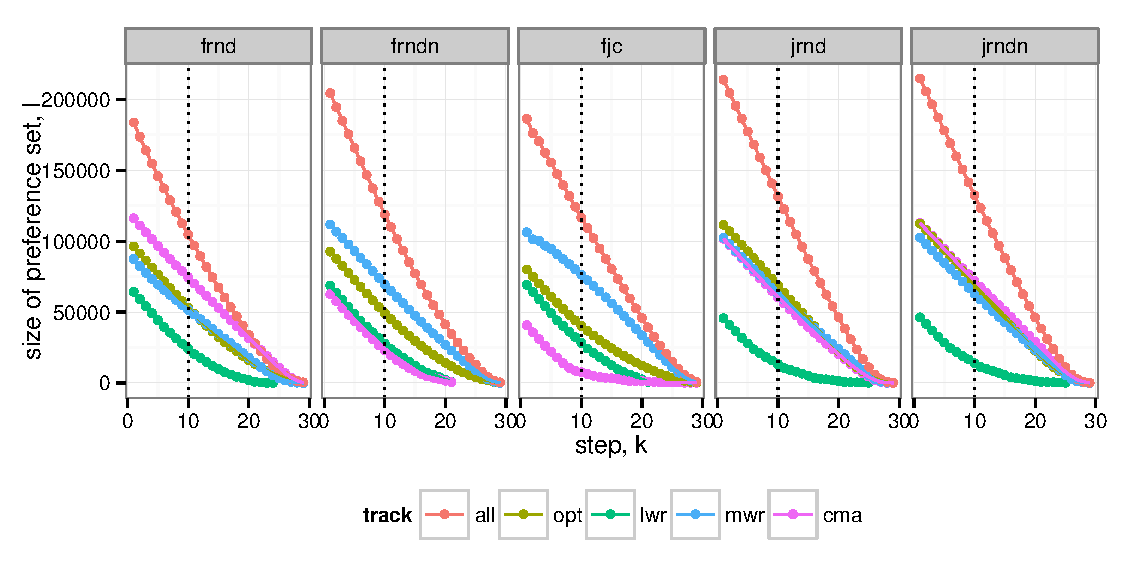
\includegraphics[width=0.8\textwidth]{figures/NUMtrinstances_d30color}
\end{figure}
\end{block}
\framebreak
\begin{block}{Linear PREF models and CMA-ES obtained weights}
\begin{figure} \centering
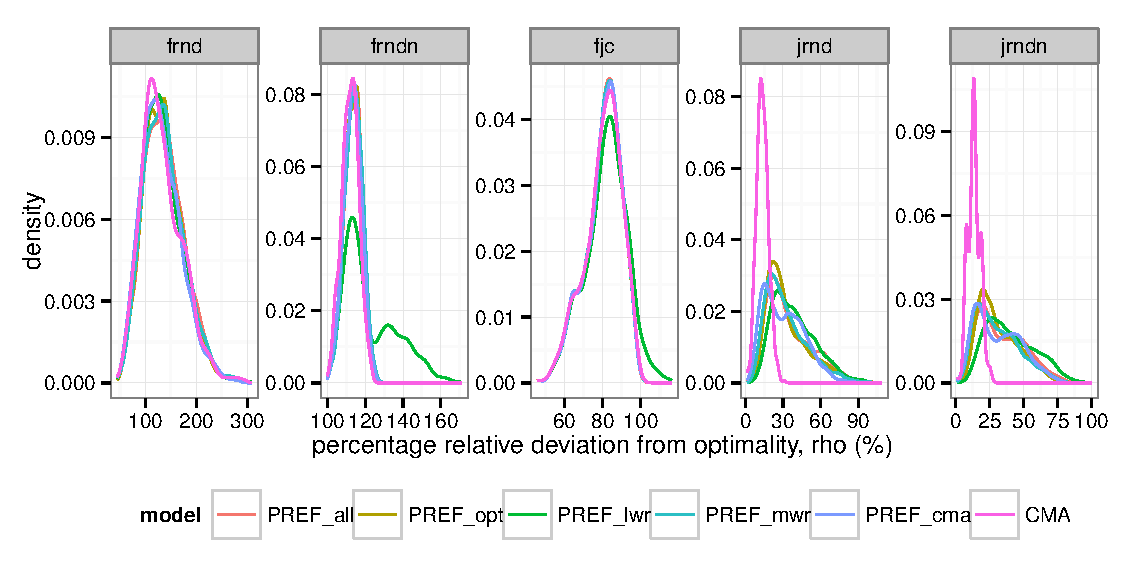
\includegraphics[width=0.8\textwidth]{figures/10x10tested4trainset}
\end{figure}
\end{block}
}

\section{Summary and conclusions}
\frame{\tableofcontents[currentsection]}

\frame[allowframebreaks]{\frametitle{Summary and conclusions}

\bi Introduced a framework for learning linear composite dispatch rules for scheduling. 
\item The approaches find linear weights by either \alert{direct optimisation with CMA-ES} or via \alert{preference learning} by collecting preference pairs whilst sampling the state space of the schedule strategically. 
\ei
\begin{block}{CMA-ES optimisation}
Benefits: 
\bi Does not rely on optimal solutions
\item Scalable
\ei 
Drawbacks:
\bi Computationally expensive .
\item Limited to linear preference function $h(\cdot)$
\ei 
Future Work:
\bi Mediate evolutionary search by use of surrogate models which indirectly estimate mean expected error w.r.t. current population without a loss in performance
\ei 
\end{block}
\begin{block}{PREF models}
Benefits:
\bi Scalable 
\item Robust to different data distributions
\ei
Drawbacks:
\bi Must know the optimal solution of the problem a priori to correctly classify optimal decisions from suboptimal ones
\ei 
Future work:
\bi Easily adaptable to non-linear preferences function, i.e. project the feature space onto a higher dimension thereby updating $h(\cdot)$ to a kernel based function which should yield lower expected $C_{\max}$ 
\ei 
\end{block}

}

\frame{
\frametitle{Thank you for your attention}
\vspace{2cm}
\begin{center} \pause {\huge\bf Questions?} \end{center}
\vfill
\begin{flushright} Helga Ingimundard\'{o}ttir, \url{hei2@hi.is}\end{flushright}
}

\end{document}